\documentclass[aspectratio=169,12pt,t]{beamer}

% --- Theme: Metropolis (modern, clean) ---
\usetheme[progressbar=frametitle,numbering=fraction,block=fill]{metropolis}

% --- Fira Sans font (install texlive-fonts-extra if missing) ---
\IfFileExists{FiraSans.sty}{\usepackage[sfdefault]{FiraSans}}{}

% --- Light background with warm accent ---
\definecolor{mDarkTeal}{RGB}{35,55,59}
\definecolor{mLightBrown}{RGB}{235,228,216}
\definecolor{mAccent}{RGB}{140,70,20}

\setbeamercolor{normal text}{fg=mDarkTeal,bg=white}
\setbeamercolor{alerted text}{fg=mAccent}
\setbeamercolor{frametitle}{bg=mDarkTeal,fg=white}
\setbeamercolor{progress bar}{fg=mAccent,bg=mLightBrown}
\setbeamercolor{title separator}{fg=mAccent}
\setbeamercolor{progress bar in head/foot}{fg=mAccent,bg=mLightBrown}
\setbeamercolor{progress bar in section page}{fg=mAccent,bg=mLightBrown}

% --- Packages ---
\usepackage[utf8]{inputenc}
\usepackage{amsmath,amssymb,amsthm}
\usepackage{mathrsfs}
\usepackage{tikz}
\usetikzlibrary{arrows.meta,positioning,calc,decorations.pathreplacing,shapes,patterns}
\usepackage{pgfplots}
\pgfplotsset{compat=1.18}

% --- Semi-transparent white highlight for text on top of background images ---
\usepackage[most]{tcolorbox}

% Inline highlight: \hl{short text}
\newtcbox{\hl}{%
  nobeforeafter, tcbox raise base,
  colback=white, opacityback=0.6,
  colframe=white, opacityframe=0,
  sharp corners, boxsep=2pt, left=3pt, right=3pt, top=2pt, bottom=2pt%
}

% Block highlight: \begin{hlbox} ... \end{hlbox}  (multi-line, paragraphs, itemize)
\newtcolorbox{hlbox}[1][]{%
  enhanced, breakable,
  colback=white, opacityback=0.6,
  colframe=white, opacityframe=0,
  boxsep=3pt, left=6pt, right=6pt, top=4pt, bottom=4pt,
  sharp corners,
  {#1}%
}

% --- Custom colors for content types ---
\definecolor{defcolor}{RGB}{25,85,120}
\definecolor{thmcolor}{RGB}{140,35,35}
\definecolor{proofcolor}{RGB}{35,100,50}
\definecolor{excolor}{RGB}{140,75,10}
\definecolor{remcolor}{RGB}{90,90,90}

% --- Beamer blocks for mathematical content types (semi-transparent) ---
\tcbset{hlblockbase/.style={
  enhanced, breakable,
  coltitle=white, fonttitle=\bfseries,
  opacitybacktitle=0.8, opacityback=0.6,
  opacityframe=0,
  sharp corners,
  boxsep=1pt, left=5pt, right=5pt, top=2pt, bottom=2pt,
  toptitle=1pt, bottomtitle=1pt
}}

\newtcolorbox{defblock}[1]{hlblockbase, title={#1},
  colbacktitle=defcolor, colback=defcolor!15, colframe=defcolor}
\newtcolorbox{thmblock}[1]{hlblockbase, title={#1},
  colbacktitle=thmcolor, colback=thmcolor!15, colframe=thmcolor}
\newtcolorbox{proofblock}[1]{hlblockbase, title={#1},
  colbacktitle=proofcolor, colback=proofcolor!15, colframe=proofcolor}
\newtcolorbox{exblock}[1]{hlblockbase, title={#1},
  colbacktitle=excolor, colback=excolor!15, colframe=excolor}
\newtcolorbox{remblock}[1]{hlblockbase, title={#1},
  colbacktitle=remcolor, colback=remcolor!15, colframe=remcolor}

% --- Metadata ---
\title{Chapter 3: Numerical Sequences and Series}
\subtitle{Section: The Number $e$}
\author{Based on Walter Rudin's \emph{Principles of Mathematical Analysis}}
\date{}

\begin{document}

% =============================================================================
% TITLE AND OUTLINE
% =============================================================================
{
\usebackgroundtemplate{%
  
\includegraphics[width=\paperwidth,height=\paperheight,keepaspectratio=false]{chapter_03_bg_00.png}%
}
\begin{frame}[plain]
  \titlepage
  \note{
    Welcome back to Chapter 3 of Principles of Mathematical Analysis.
    In this short but rewarding section we meet one of the most
    important constants in all of mathematics, the number "e".
    Everything we need is already in our hands: we have a solid theory
    of series, we know the geometric series, and we have upper and
    lower limits. We will put those tools to work. We will define "e"
    as the sum of a rapidly converging series, then prove that the
    very same number arises from a completely different limit, the
    limit of one plus one over "n", raised to the power "n". Finally,
    we will use a sharp estimate on how fast the series converges to
    prove something striking: the number "e" is irrational. Let's
    begin.
  }
\end{frame}
}

{
\usebackgroundtemplate{%
  
\includegraphics[width=\paperwidth,height=\paperheight,keepaspectratio=false]{chapter_03_bg_01.png}%
}
\begin{frame}[c]{Outline}
  \begin{center}
    \tableofcontents
  \end{center}
  \note{
    Here is our plan. We start with motivation: why "e" deserves its
    own section and what makes it special. Then we give the official
    definition of "e" as an infinite series and check that the series
    actually converges. Next comes the first big theorem, which shows
    that "e" is also the limit of one plus one over "n" to the "n".
    After that we measure how quickly the defining series converges,
    obtaining a clean error estimate. That estimate is the key to the
    final result, the proof that "e" is irrational. We close with a
    summary of what we have learned.
  }
\end{frame}

% =============================================================================
\section{Motivation}
% =============================================================================

% --- Build 1/3 ---
\begin{frame}{Why the Number $e$?}
  \begin{hlbox}
  \begin{itemize}
    \item $e$ is one of the \alert{fundamental constants} of mathematics
  \end{itemize}
  \end{hlbox}

  \note{
    Let's set the stage. The number "e" is one of the fundamental
    constants of mathematics, sitting alongside the number pi in
    importance. It is the natural base for exponentials and
    logarithms, it governs compound growth and decay, and it appears
    throughout analysis, probability, and number theory. Its
    numerical value is roughly 2.718. But a number this important
    deserves a precise definition, not just a decimal approximation.
    Next, let's see what tools we will use to pin it down.
  }
\end{frame}

% --- Build 2/3 ---
\begin{frame}{Why the Number $e$?}
  \begin{hlbox}
  \begin{itemize}
    \item $e$ is one of the \alert{fundamental constants} of mathematics
    \item We now have the tools to define it \alert{rigorously}: series, limits
  \end{itemize}
  \end{hlbox}

  \note{
    Here is the good news. We do not need any new machinery. Over the
    last several sections we built a careful theory of infinite
    series, we analyzed the geometric series in detail, and we
    introduced upper and lower limits. Those are exactly the tools
    needed to define "e" rigorously and to study it. This section is
    really a showcase: it demonstrates how the abstract theory pays
    off on a concrete and famous example. Next, let's preview the two
    surprises waiting for us.
  }
\end{frame}

% --- Build 3/3 ---
\begin{frame}{Why the Number $e$?}
  \begin{hlbox}
  \begin{itemize}
    \item $e$ is one of the \alert{fundamental constants} of mathematics
    \item We now have the tools to define it \alert{rigorously}: series, limits
    \item Two surprises ahead:
      \begin{itemize}
        \item $e$ is also a \alert{limit}: $\lim\left(1 + \tfrac{1}{n}\right)^n$
        \item $e$ is \alert{irrational}
      \end{itemize}
  \end{itemize}
  \end{hlbox}

  \note{
    This section holds two surprises. The first is that "e", which we
    will define as an infinite series, turns out to equal a
    completely different-looking limit: the limit of one plus one
    over "n", all raised to the power "n". The fact that these two
    processes land on the same number is not obvious, and the proof
    is a beautiful exercise in handling limits. The second surprise
    is that "e" is irrational. It cannot be written as a ratio of two
    integers. We will prove both of these. Let's start by writing
    down the definition.
  }
\end{frame}
}

{
\usebackgroundtemplate{%
  
\includegraphics[width=\paperwidth,height=\paperheight,keepaspectratio=false]{chapter_03_bg_02.png}%
}
% =============================================================================
\section{Defining the Number $e$}
% =============================================================================

\begin{frame}{Definition 3.30: The Number $e$}
  \begin{defblock}{Definition 3.30}
    \[
      e = \sum_{n=0}^{\infty} \frac{1}{n!}.
    \]
  \end{defblock}

  \vspace{0.6em}
  \begin{hlbox}
  \textbf{Factorial convention:}
  \[
    n! = 1 \cdot 2 \cdot 3 \cdots n \quad (n \geq 1), \qquad 0! = 1.
  \]
  \end{hlbox}

  \note{
    Here is the official definition. The number "e" is defined to be
    the sum of the infinite series whose terms are one over "n"
    factorial, summed from "n" equal zero to infinity. So the terms
    are one over zero factorial, one over one factorial, one over two
    factorial, and so on. We need a convention for the factorial. For
    "n" at least one, "n" factorial is the product one times two
    times three, up to "n". And by convention, zero factorial is
    defined to be one. With that convention the first two terms of
    the series are both equal to one. But before we can call this a
    definition, we must check that the series actually converges.
    Let's do that next.
  }
\end{frame}

% --- Build 1/3: convergence ---
\begin{frame}{Does the Series Converge?}
  \begin{hlbox}
  Write the $n$-th partial sum:
  \[
    s_n = 1 + 1 + \frac{1}{1\cdot 2} + \frac{1}{1\cdot 2\cdot 3}
         + \cdots + \frac{1}{1\cdot 2 \cdots n}.
  \]
  \end{hlbox}

  \note{
    To check convergence we look at the partial sums. The partial sum
    "s" sub "n" is what you get by adding up the first several terms
    of the series: one, plus one, plus one over one times two, plus
    one over one times two times three, and so on, up to one over the
    product of all the integers from one to "n". Because every term
    is positive, the partial sums keep increasing as we include more
    of them. And we proved earlier that a series of nonnegative terms
    converges exactly when its partial sums stay bounded above. So the
    whole question of convergence reduces to a single thing: can we
    find a ceiling that the partial sums never rise past? Next, let's
    compare term by term with a geometric series.
  }
\end{frame}

% --- Build 2/3: comparison ---
\begin{frame}{Does the Series Converge?}
  \begin{hlbox}
  Write the $n$-th partial sum:
  \[
    s_n = 1 + 1 + \frac{1}{1\cdot 2} + \frac{1}{1\cdot 2\cdot 3}
         + \cdots + \frac{1}{1\cdot 2 \cdots n}.
  \]
  Compare each term: for $k \geq 1$, \quad $\dfrac{1}{k!} \leq \dfrac{1}{2^{\,k-1}}$.
  \[
    s_n < 1 + 1 + \frac{1}{2} + \frac{1}{2^2} + \cdots + \frac{1}{2^{n-1}}.
  \]
  \end{hlbox}

  \note{
    Now the key comparison. Each factorial "k" factorial is a product
    of "k" numbers, and from the second factor onward every factor is
    at least two. So "k" factorial is at least two to the power "k"
    minus one. Turning that around, one over "k" factorial is at most
    one over two to the "k" minus one. Replacing every term of "s"
    sub "n" by the corresponding power of one half gives a strictly
    larger sum, shown on the slide. We have bounded our partial sum
    above by a partial sum of the geometric series with ratio one
    half. Next, let's add up that geometric piece.
  }
\end{frame}

% --- Build 3/3: bound ---
\begin{frame}{Does the Series Converge?}
  \begin{hlbox}
  Write the $n$-th partial sum:
  \[
    s_n = 1 + 1 + \frac{1}{1\cdot 2} + \frac{1}{1\cdot 2\cdot 3}
         + \cdots + \frac{1}{1\cdot 2 \cdots n}.
  \]
  Compare each term: for $k \geq 1$, \quad $\dfrac{1}{k!} \leq \dfrac{1}{2^{\,k-1}}$.
  \[
    s_n < 1 + \underbrace{1 + \frac{1}{2} + \cdots + \frac{1}{2^{n-1}}}_{<\, 2}
        \; < \; 3.
  \]
  \alert{Bounded above by $3$} $\;\Longrightarrow\;$ the series \alert{converges}.
  \end{hlbox}

  \note{
    The geometric part, one plus one half plus one quarter and so on,
    is a partial sum of a geometric series with ratio one half, and
    that whole geometric series sums to two. So the bracketed piece
    is less than two. Adding the leading one, every partial sum "s"
    sub "n" is less than three. The partial sums are increasing and
    bounded above by three, so the series converges. The definition
    of "e" makes sense, and we already know "e" lies somewhere
    between two and three. Next, let's picture this convergence on a
    number line.
  }
\end{frame}

\begin{frame}{The Partial Sums Close In on $e$}
  \begin{center}
  \begin{tikzpicture}[scale=1.0]
    % number line
    \draw[->] (-0.3,0) -- (11,0);
    \foreach \v/\x in {1/0, 2/5, 3/10}{
      \draw (\x,0.12) -- (\x,-0.12) node[below]{\footnotesize $\v$};
    }
    % partial sums: s0=1, s1=2, s2=2.5, s3=2.6667, s4=2.7083
    % map value v -> x = (v-1)*5
    \fill[defcolor] (0,0) circle (2.4pt) node[above=3pt]{\scriptsize $s_0$};
    \fill[defcolor] (5,0) circle (2.4pt) node[above=3pt]{\scriptsize $s_1$};
    \fill[defcolor] (7.5,0) circle (2.4pt) node[above=9pt]{\scriptsize $s_2$};
    \fill[defcolor] (8.333,0) circle (2.4pt) node[above=3pt]{\scriptsize $s_3$};
    \fill[defcolor] (8.542,0) circle (2.4pt);
    % e at (2.71828-1)*5 = 8.5914
    \draw[thmcolor, very thick] (8.5914,0.35) -- (8.5914,-0.35);
    \node[thmcolor] at (8.5914,0.7) {$e$};
    % bound at 3
    \draw[mAccent, thick, dashed] (10,0.55) -- (10,-0.2);
    \node[mAccent, align=center] at (10,0.95) {\scriptsize bound};
  \end{tikzpicture}
  \end{center}

  \vspace{0.4em}
  \begin{center}
    \hl{\textbf{Increasing} and \textbf{bounded} $\;\Longrightarrow\;$
    $s_n \uparrow e$, \quad with $2 < e < 3$.}
  \end{center}

  \note{
    This picture shows the partial sums marching toward "e" on the
    number line. The blue dots are the partial sums "s" sub zero, "s"
    sub one, "s" sub two, "s" sub three, and so on. The first jump,
    from "s" sub zero to "s" sub one, is large, but after that the
    dots crowd together very quickly and pile up just below the dark
    red mark labelled "e". The dashed orange line on the right at the
    value three is the upper bound we just proved. Because the
    sequence is increasing and never crosses three, it converges, and
    its limit "e" sits between two and three. Notice how rapidly the
    dots converge; that rapid convergence is worth a closer look.
  }
\end{frame}

\begin{frame}{A Series That Converges Very Fast}
  \begin{remblock}{Remark}
    The series $\displaystyle\sum \frac{1}{n!}$ converges \alert{very rapidly}.
  \end{remblock}

  \vspace{0.5em}
  \begin{hlbox}
  \begin{itemize}
    \item Each term shrinks faster than any geometric series.
    \item This lets us compute $e$ with \alert{great accuracy}.
    \item We will make ``rapidly'' precise with a sharp \alert{error bound}.
  \end{itemize}
  \end{hlbox}

  \note{
    Before moving on, one observation worth keeping in mind. The
    series for "e" converges very rapidly, even faster than a
    geometric series, because the factorial in the denominator grows
    faster than any fixed power. Practically, this means that adding
    just a handful of terms already gives "e" to many decimal places.
    We will make the word rapidly completely precise a little later,
    when we derive a sharp bound on the error. For now, let's turn to
    the first major theorem, which reveals "e" hiding inside a very
    different limit.
  }
\end{frame}
}

{
\usebackgroundtemplate{%
  
\includegraphics[width=\paperwidth,height=\paperheight,keepaspectratio=false]{chapter_03_bg_03.png}%
}
% =============================================================================
\section{$e$ as a Limit}
% =============================================================================

\begin{frame}{Theorem 3.31: $e$ as a Limit}
  \begin{thmblock}{Theorem 3.31}
    \[
      \lim_{n \to \infty} \left(1 + \frac{1}{n}\right)^{n} = e.
    \]
  \end{thmblock}

  \vspace{0.4em}
  \begin{hlbox}
  \textbf{Key idea:} The number defined by a \emph{series} also arises
  from a \emph{limit process}.
  \end{hlbox}

  \vspace{0.3em}
  \begin{center}
  \begin{tikzpicture}[scale=1.0]
    \draw[->] (-0.3,0) -- (9.5,0);
    \foreach \v/\x in {2/0, 2.5/6}{
      \draw (\x,0.1) -- (\x,-0.1) node[below]{\footnotesize $\v$};
    }
    \fill[defcolor] (0,0) circle (2.2pt) node[above=3pt]{\scriptsize $t_1$};
    \fill[defcolor] (3,0) circle (2.2pt) node[above=3pt]{\scriptsize $t_2$};
    \fill[defcolor] (4.44,0) circle (2.2pt) node[above=3pt]{\scriptsize $t_3$};
    \fill[defcolor] (5.86,0) circle (2.2pt) node[above=3pt]{\scriptsize $t_5$};
    \fill[defcolor] (7.13,0) circle (2.2pt) node[above=3pt]{\scriptsize $t_{10}$};
    \draw[thmcolor, very thick] (8.62,0.34) -- (8.62,-0.34);
    \node[thmcolor] at (8.62,0.62) {$e$};
  \end{tikzpicture}
  \end{center}

  \vspace{0.1em}
  \begin{center}
    \hl{\footnotesize Even $t_{10}\approx 2.594$: this limit creeps
    toward $e$ \emph{slowly}.}
  \end{center}

  \note{
    Here is the first theorem. It says that the limit, as "n" goes to
    infinity, of one plus one over "n", all raised to the power "n",
    is exactly the number "e" we just defined. The number line lets
    you watch it happen. The blue dots are the values "t" sub one,
    "t" sub two, "t" sub three, "t" sub five, and "t" sub ten, and
    they climb steadily from left to right toward the dark red mark
    at "e". Notice how slowly they climb: even "t" sub ten has only
    reached about two point five nine, while "e" is about two point
    seven two. So this limit creeps toward "e", unlike the series,
    which raced ahead. Still, the theorem is remarkable: a sum of
    reciprocal factorials, and a shrinking base raised to a growing
    power, land on the very same number. The proof is a fine
    illustration of working with limits. Let's lay out the strategy.
  }
\end{frame}

\begin{frame}{Proof Strategy: Theorem 3.31}
  \begin{hlbox}
  \textbf{Goal:} Show $t_n := \left(1 + \tfrac{1}{n}\right)^n \to e$.

  \vspace{0.8em}
  \textbf{Approach --- squeeze between upper and lower limits:}
  \begin{enumerate}
    \item Expand $t_n$ with the \alert{binomial theorem}.
    \item Compare with $s_n$ term by term: $t_n \leq s_n$,
          so $\displaystyle\limsup_{n\to\infty} t_n \leq e$.
    \item Bound $t_n$ from \emph{below} by a truncated sum;
          deduce $\displaystyle e \leq \liminf_{n\to\infty} t_n$.
    \item Combine: $\limsup t_n \leq e \leq \liminf t_n$ forces the limit.
  \end{enumerate}
  \end{hlbox}

  \note{
    Before the formal proof, here is the plan. We name the sequence:
    "t" sub "n" is one plus one over "n" to the "n". The strategy is
    a squeeze, but a squeeze on the upper and lower limits rather than
    on the sequence directly. First, we expand "t" sub "n" using the
    binomial theorem. Second, we compare it term by term with the
    partial sum "s" sub "n" of the series for "e"; this gives "t" sub
    "n" at most "s" sub "n", which pushes the upper limit of "t" sub
    "n" below "e". Third, we bound "t" sub "n" from below by keeping
    only finitely many terms; this pushes the lower limit of "t" sub
    "n" above "e". Finally, since the upper limit is at most "e" and
    the lower limit is at least "e", the sequence must converge to
    "e". Let's begin.
  }
\end{frame}

\begin{frame}{Proof of Theorem 3.31 --- Step 1: Setup}
  \begin{proofblock}{Step 1: Name the two sequences}
    \[
      s_n = \sum_{k=0}^{n} \frac{1}{k!}, \qquad
      t_n = \left(1 + \frac{1}{n}\right)^{n}.
    \]
  \end{proofblock}

  \vspace{0.5em}
  \hl{We already know $s_n \to e$. \quad Goal: show $t_n \to e$ as well.}

  \note{
    We begin by giving names to the two players. The sequence "s" sub
    "n" is the partial sum of the series for "e", the sum of one over
    "k" factorial for "k" from zero to "n". We have already shown
    this converges to "e". The sequence "t" sub "n" is the one in the
    theorem, one plus one over "n" raised to the power "n". Our goal
    is to show that "t" sub "n" also converges to "e". The link
    between them will come from expanding "t" sub "n". Next, let's
    apply the binomial theorem.
  }
\end{frame}

\begin{frame}{Proof of Theorem 3.31 --- Step 2: Binomial Expansion}
  \begin{proofblock}{Step 2: Expand $t_n$ by the binomial theorem}
    \begin{align*}
      t_n = 1 + \frac{n}{1!} \cdot \frac{1}{n} &+ \frac{n (n-1)}{2!} \cdot \frac{1}{n^2}
              + \cdots + \frac{n (n-1) \cdots 1}{n!} \cdot \frac{1}{n^n} = \\[2pt]
            1 + 1 &+ \frac{1}{2!}\left(1 - \frac{1}{n}\right)
             + \frac{1}{3!}\left(1 - \frac{1}{n}\right)\left(1 - \frac{2}{n}\right) + \cdots\\[2pt]
           &+ \frac{1}{n!}\left(1 - \frac{1}{n}\right)\left(1 - \frac{2}{n}\right)
             \cdots\left(1 - \frac{n-1}{n}\right).
    \end{align*}
  \end{proofblock}

  \vspace{0.4em}
  \begin{hlbox}
  Each term mirrors a term of $s_n$, but \alert{dampened} by factors
  $\left(1 - \tfrac{j}{n}\right) \leq 1$.
  \end{hlbox}

  \note{
    Step two: expand "t" sub "n" using the binomial theorem. The
    first line on the slide is the raw expansion. A typical term
    there is a binomial coefficient, that product of descending
    integers divided by "k" factorial, multiplied by one over "n"
    raised to the power "k". The second and third lines tidy each
    term up. The trick is to spread the powers of "n" in the
    denominator across the descending factors in the numerator: the
    product "n" times "n" minus one, and so on, divided by "n" to the
    "k", turns into one, times one minus one over "n", times one
    minus two over "n", and so forth. So every term collapses to one
    over "k" factorial multiplied by a string of factors of the form
    one minus "j" over "n". Now look at the shape of the result. Term
    by term it mirrors the partial sum "s" sub "n", the very same one
    over "k" factorial appearing, except each term is now dampened by
    those factors one minus "j" over "n", every one of which is
    positive and at most one. So each term of "t" sub "n" is a
    shrunken copy of the matching term of "s" sub "n". Let's exploit
    that comparison next.
  }
\end{frame}

\begin{frame}{Proof of Theorem 3.31 --- Step 3: The Upper Limit}
  \begin{hlbox}
  Since every factor $\left(1 - \tfrac{j}{n}\right) \leq 1$:
  \[
    t_n \leq s_n \qquad \text{for all } n.
  \]
  Taking upper limits (Theorem 3.19):
  \begin{equation*}
    \limsup_{n \to \infty} t_n \;\leq\; e. \tag{14}
  \end{equation*}
  \end{hlbox}

  \note{
    Step three. Because each damping factor is at most one,
    discarding all of them only increases the value. Term by term,
    "t" sub "n" is less than or equal to "s" sub "n", for every "n".
    Now we take upper limits on both sides. By Theorem 3.19, if one
    sequence stays below another, then its upper limit stays below
    the limit of the other. The sequence "s" sub "n" converges to
    "e", so the upper limit of "t" sub "n" is at most "e". Call this
    equation 14. That is one half of the squeeze. Next, we need a
    lower bound, and that takes a slightly cleverer move.
  }
\end{frame}

\begin{frame}{Proof of Theorem 3.31 --- Step 4: Truncate from Below}
  \begin{hlbox}
  \textbf{Strategy:} keep only the first $m+1$ terms ($m$ fixed). For $n \geq m$,
  \[
    t_n \;\geq\; 1 + 1 + \frac{1}{2!}\left(1 - \frac{1}{n}\right)
       + \cdots + \frac{1}{m!}\left(1 - \frac{1}{n}\right)\cdots\left(1 - \frac{m-1}{n}\right).
  \]
  \alert{All discarded terms are positive}, so dropping them lowers the value.
  \end{hlbox}

  \note{
    Step four. For the lower bound we use a different idea. The
    expansion of "t" sub "n" has lots of terms, and every single one
    of them is positive. So if we throw away all the terms past a
    fixed cutoff "m", the sum can only get smaller. That gives the
    inequality on the slide: for "n" at least "m", "t" sub "n" is at
    least the truncated sum that keeps only the first "m" plus one
    terms. The point of freezing "m" is that the truncated sum has a
    fixed, finite number of terms, no matter how large "n" gets. That
    is what makes the next step possible. Let's take the limit in
    "n".
  }
\end{frame}

\begin{frame}{Proof of Theorem 3.31 --- Step 5: Let $n \to \infty$, $m$ Fixed}
  \begin{hlbox}
  In the truncated sum, let $n \to \infty$ with $m$ \emph{fixed}.
  Each factor $\left(1 - \tfrac{j}{n}\right) \to 1$:
  \[
    \liminf_{n \to \infty} t_n \;\geq\;
       1 + 1 + \frac{1}{2!} + \cdots + \frac{1}{m!} \;=\; s_m.
  \]
  Hence \quad $s_m \leq \displaystyle\liminf_{n \to \infty} t_n$ \quad for every $m$.
  \end{hlbox}

  \note{
    Step five. Now hold "m" fixed and let "n" go to infinity in the
    truncated lower bound. The truncated sum has only finitely many
    terms, and in each one the damping factors, one minus "j" over
    "n", all tend to one as "n" grows. So the whole truncated sum
    tends to one plus one plus one over two factorial, up to one over
    "m" factorial, which is exactly the partial sum "s" sub "m". Since
    "t" sub "n" stays above the truncated sum, its lower limit stays
    above the limiting value. We conclude that "s" sub "m" is less
    than or equal to the lower limit of "t" sub "n", and this holds
    for every fixed "m". One more limit to take.
  }
\end{frame}

\begin{frame}{Proof of Theorem 3.31 --- Step 6: Let $m \to \infty$}
  \begin{hlbox}
  We have $s_m \leq \liminf_{n\to\infty} t_n$ for \emph{every} $m$.
  Let $m \to \infty$: $s_m \to e$, so
  \begin{equation*}
    e \;\leq\; \liminf_{n \to \infty} t_n. \tag{15}
  \end{equation*}
  \end{hlbox}

  \vspace{0.5em}
  \begin{remblock}{Recall: Theorem 3.19}
    If $s_m \leq c$ for all $m$ and $s_m \to e$, then $e \leq c$.
  \end{remblock}

  \note{
    Step six. We have just shown that every partial sum "s" sub "m"
    lies below the lower limit of "t" sub "n". The right-hand side is
    one fixed number; it does not depend on "m". So we may let "m" go
    to infinity. The partial sums "s" sub "m" converge to "e", and a
    limit of quantities all sitting below a fixed bound cannot exceed
    that bound. This is the principle recalled in the gray box, a
    consequence of Theorem 3.19. Therefore "e" is less than or equal
    to the lower limit of "t" sub "n". Call this equation 15. We now
    have both halves of the squeeze. Let's put them together.
  }
\end{frame}

\begin{frame}{Proof of Theorem 3.31 --- Conclusion}
  \begin{center}
  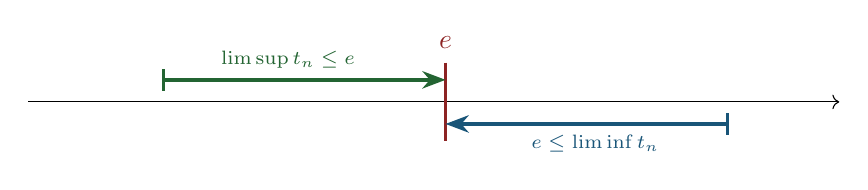
\begin{tikzpicture}[scale=1.0]
    \draw[->] (-0.3,0) -- (10,0);
    % e mark
    \draw[thmcolor, very thick] (5,0.5) -- (5,-0.5);
    \node[thmcolor, above] at (5,0.55) {$e$};
    % limsup <= e  (arrow from left up to e)
    \draw[proofcolor, very thick, {Bar}-{Stealth}] (1.4,0.28) -- (5,0.28);
    \node[proofcolor, above, font=\scriptsize] at (3.0,0.30) {$\limsup t_n \leq e$};
    % e <= liminf  (arrow from e to the right)
    \draw[defcolor, very thick, {Stealth}-{Bar}] (5,-0.28) -- (8.6,-0.28);
    \node[defcolor, below, font=\scriptsize] at (6.9,-0.30) {$e \leq \liminf t_n$};
  \end{tikzpicture}
  \end{center}

  \begin{hlbox}
  \[
    e \;\overset{(15)}{\leq}\; \liminf_{n\to\infty} t_n \;\leq\; \limsup_{n\to\infty} t_n
    \;\overset{(14)}{\leq}\; e.
  \]
  All equal $e$, so \quad $\boxed{\;\lim\limits_{n\to\infty} t_n = e\;}$ \qquad $\blacksquare$
  \end{hlbox}

  \note{
    Now we combine equations 14 and 15. The diagram shows the
    squeeze. The green arrow on top says the upper limit of "t" sub
    "n" sits at or below "e". The blue arrow underneath says "e" sits
    at or below the lower limit of "t" sub "n". Now read the chain of
    inequalities on the slide. We start at "e". By equation 15, "e"
    is at most the lower limit. For any sequence the lower limit is
    always at most the upper limit, and that holds automatically. And
    by equation 14, the upper limit is at most "e". So the chain
    begins at "e" and ends at "e", with the lower and upper limits
    trapped in between. Everything in the chain is therefore pinned
    to the single value "e". And when the lower and upper limits of a
    sequence agree, the sequence itself converges to that common
    value. Therefore "t" sub "n" converges to "e", and the theorem is
    proved. Next, let's measure exactly how fast the original series
    converges.
  }
\end{frame}
}

{
\usebackgroundtemplate{%
  
\includegraphics[width=\paperwidth,height=\paperheight,keepaspectratio=false]{chapter_03_bg_04.png}%
}
% =============================================================================
\section{How Fast the Series Converges}
% =============================================================================

\begin{frame}{Estimating the Error $e - s_n$}
  \begin{hlbox}
  How close is the partial sum $s_n$ to $e$? Look at the leftover tail:
  \[
    e - s_n = \frac{1}{(n+1)!} + \frac{1}{(n+2)!} + \frac{1}{(n+3)!} + \cdots
  \]
  \end{hlbox}

  \note{
    We promised to make the word rapidly precise. The error in using
    the partial sum "s" sub "n" as an approximation to "e" is exactly
    the tail of the series: the sum of all the terms we left out.
    That tail is one over "n" plus one factorial, plus one over "n"
    plus two factorial, plus one over "n" plus three factorial, and
    so on. Since every term is positive, the error is certainly
    positive; "s" sub "n" underestimates "e". The question is how
    large the tail can be. Let's bound it.
  }
\end{frame}

\begin{frame}{A Geometric Bound on the Tail}
  \begin{hlbox}
  Factor out $\dfrac{1}{(n+1)!}$ and overestimate each factorial ratio:
  \[
    e - s_n < \frac{1}{(n+1)!}\left\{1 + \frac{1}{n+1} + \frac{1}{(n+1)^2} + \cdots\right\}
            = \frac{1}{n!\,n}.
  \]
  \begin{equation*}
    \boxed{\,0 < e - s_n < \dfrac{1}{n!\,n}\,} \tag{16}
  \end{equation*}
  \end{hlbox}

  \note{
    Here is the trick. Factor one over "n" plus one factorial out of
    every term of the tail. The next term then carries a factor one
    over "n" plus two factorial divided by "n" plus one factorial,
    which is one over "n" plus two; we overestimate that by one over
    "n" plus one. The term after that gets overestimated by one over
    "n" plus one squared, and so on. So the tail is less than one
    over "n" plus one factorial times a geometric series with ratio
    one over "n" plus one. That geometric series sums neatly, and
    after simplification the whole bound collapses to one over "n"
    factorial times "n". This is equation 16: the error is positive
    and strictly less than one over "n" factorial times "n". Let's
    see what that means in practice.
  }
\end{frame}

\begin{frame}{The Series Converges Astonishingly Fast}
  \begin{exblock}{Example: $n = 10$}
    \[
      0 < e - s_{10} < \frac{1}{10!\cdot 10} = \frac{1}{36{,}288{,}000} < 10^{-7}.
    \]
  \end{exblock}

  \vspace{0.5em}
  \begin{hlbox}
  \begin{itemize}
    \item Just \alert{11 terms} pin down $e$ to better than 7 decimals.
    \item Estimate (16) also has \alert{theoretical} value --- see next section.
  \end{itemize}
  \end{hlbox}

  \note{
    Let's put a number on it. Take "n" equal to ten. Then the error
    "e" minus "s" sub ten is less than one over ten factorial times
    ten. Ten factorial is about three point six million, so the
    denominator exceeds thirty six million, and the error is smaller
    than ten to the minus seven. In words: adding just eleven terms
    of the series, the terms up through one over ten factorial,
    already determines "e" to better than seven decimal places. That
    is what rapid convergence means here. But estimate 16 is not only
    useful for computation. It also has real theoretical power, and
    in the next section we use it to prove that "e" is irrational.
  }
\end{frame}
}

{
\usebackgroundtemplate{%
  
\includegraphics[width=\paperwidth,height=\paperheight,keepaspectratio=false]{chapter_03_bg_05.png}%
}
% =============================================================================
\section{$e$ is Irrational}
% =============================================================================

\begin{frame}{Theorem 3.32: $e$ is Irrational}
  \begin{thmblock}{Theorem 3.32}
    $e$ is \alert{irrational}.
  \end{thmblock}

  \vspace{0.6em}
  \begin{hlbox}
  \textbf{Meaning:} there are \emph{no} integers $p, q$ with
  $e = \dfrac{p}{q}$.

  \vspace{0.4em}
  \textbf{Technique:} proof by contradiction, powered by estimate (16).
  \end{hlbox}

  \note{
    Now the second surprise. Theorem 3.32 states that "e" is
    irrational. That means "e" cannot be written as a fraction "p"
    over "q" with "p" and "q" integers. Its decimal expansion never
    settles into a repeating pattern. The proof is short and elegant.
    It is a proof by contradiction: we assume "e" is rational and
    derive an impossibility. The engine driving the contradiction is
    the error estimate 16 we just proved. Let's outline the
    argument.
  }
\end{frame}

\begin{frame}{Proof Strategy: Theorem 3.32}
  \begin{hlbox}
  \textbf{Goal:} rule out $e = p/q$ with $p, q$ positive integers.

  \vspace{0.8em}
  \textbf{Approach:}
  \begin{enumerate}
    \item Assume for contradiction $e = p/q$.
    \item Multiply estimate (16) by $q!$: trap $q!(e - s_q)$ in $(0, 1)$.
    \item Show $q!(e - s_q)$ is an \alert{integer}.
    \item An integer strictly between $0$ and $1$ --- impossible!
  \end{enumerate}
  \end{hlbox}

  \note{
    Here is the high-level strategy. We want to rule out writing "e"
    as "p" over "q" with "p" and "q" positive integers. We assume,
    for contradiction, that such a representation exists. Then we
    take the error estimate 16 and multiply it through by "q"
    factorial; this traps the quantity "q" factorial times the
    difference "e" minus "s" sub "q" strictly between zero and one.
    Next we show, using the assumption, that this same quantity is in
    fact a whole number, an integer. But there is no integer strictly
    between zero and one. That contradiction kills the assumption.
    Let's carry it out.
  }
\end{frame}

\begin{frame}{Proof of Theorem 3.32 --- Step 1: Apply Estimate (16)}
  \begin{proofblock}{Step 1: Assume $e = p/q$ and scale (16) by $q!$}
    Suppose $e = p/q$ with $p, q$ positive integers. From (16):
    \begin{equation*}
      0 < q!\,(e - s_q) < \frac{1}{q}. \tag{17}
    \end{equation*}
  \end{proofblock}

  \vspace{0.4em}
  \begin{hlbox}
  Since $q \geq 1$, the upper bound $\tfrac{1}{q} \leq 1$:
  \quad $q!(e - s_q) \in (0, 1)$.
  \end{hlbox}

  \note{
    Step one. Assume "e" equals "p" over "q", with "p" and "q"
    positive integers. Estimate 16, applied with "n" equal to "q",
    says that "e" minus "s" sub "q" lies strictly between zero and
    one over "q" factorial times "q". Multiply that whole inequality
    by "q" factorial. The result, equation 17, says that "q"
    factorial times the difference "e" minus "s" sub "q" lies
    strictly between zero and one over "q". Since "q" is at least
    one, one over "q" is at most one. So this quantity is trapped
    strictly between zero and one. Remember that fact. Next, we show
    the very same quantity is an integer.
  }
\end{frame}

\begin{frame}{Proof of Theorem 3.32 --- Step 2: $q!\,e$ is an Integer}
  \begin{hlbox}
  Under the assumption $e = p/q$:
  \[
    q!\,e = q!\cdot\frac{p}{q} = (q-1)!\;p \;\in\; \mathbb{Z}.
  \]
  The factor $q$ in the denominator is cancelled by $q!$.
  \end{hlbox}

  \note{
    Step two. Look at "q" factorial times "e". Under our assumption
    "e" is "p" over "q", so "q" factorial times "e" is "q" factorial
    times "p" divided by "q". But "q" factorial contains the factor
    "q", so the "q" in the denominator cancels, leaving "q" minus one
    factorial times "p". That is a product of integers, hence an
    integer. So "q" factorial times "e" is a whole number. This is
    the only place where the rationality assumption is used. Next, we
    handle the other piece.
  }
\end{frame}

\begin{frame}{Proof of Theorem 3.32 --- Step 3: $q!\,s_q$ is an Integer}
  \begin{hlbox}
  \[
    q!\,s_q = q!\left(1 + 1 + \frac{1}{2!} + \cdots + \frac{1}{q!}\right).
  \]
  Each term $\dfrac{q!}{k!}$ with $0 \leq k \leq q$ is an integer
  $\;\Longrightarrow\; q!\,s_q \in \mathbb{Z}$.
  \end{hlbox}

  \note{
    Step three. Now consider "q" factorial times the partial sum "s"
    sub "q". The partial sum is one plus one plus one over two
    factorial, up to one over "q" factorial. Multiply each term by
    "q" factorial. A typical term becomes "q" factorial divided by
    "k" factorial, with "k" running from zero up to "q". Since "k" is
    at most "q", that quotient is a product of consecutive integers,
    so every term is an integer. A sum of integers is an integer.
    Therefore "q" factorial times "s" sub "q" is a whole number too.
    No assumption was needed here; this part is just arithmetic.
    Let's collect the pieces.
  }
\end{frame}

\begin{frame}{Proof of Theorem 3.32 --- Step 4: The Contradiction}
  \begin{hlbox}
  Both $q!\,e$ and $q!\,s_q$ are integers, hence so is their difference:
  \[
    q!\,(e - s_q) = q!\,e - q!\,s_q \;\in\; \mathbb{Z}.
  \]
  But (17) says \quad $0 < q!\,(e - s_q) < 1$.
  \end{hlbox}

  \vspace{0.4em}
  \begin{center}
  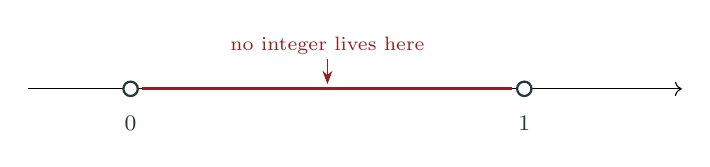
\begin{tikzpicture}[scale=1.0]
    \draw[->] (-0.3,0) -- (8,0);
    % shaded open interval
    \draw[thmcolor, very thick] (1.15,0) -- (5.85,0);
    % open circles at 0 and 1 (endpoints excluded)
    \draw[mDarkTeal, thick, fill=white] (1,0) circle (2.6pt) node[below=6pt]{\footnotesize $0$};
    \draw[mDarkTeal, thick, fill=white] (6,0) circle (2.6pt) node[below=6pt]{\footnotesize $1$};
    \node[thmcolor, align=center, font=\scriptsize] at (3.5,0.55)
      {no integer lives here};
    \draw[thmcolor, -{Stealth}] (3.5,0.38) -- (3.5,0.06);
  \end{tikzpicture}
  \end{center}

  \begin{center}
    \hl{\alert{An integer strictly between $0$ and $1$ --- contradiction!} \quad $\blacksquare$}
  \end{center}

  \note{
    Step four ties it all together. From steps two and three, both
    "q" factorial times "e" and "q" factorial times "s" sub "q" are
    integers. Their difference is "q" factorial times the quantity
    "e" minus "s" sub "q", so that difference is an integer as well.
    But equation 17 told us this very quantity lies strictly between
    zero and one. The picture makes the clash vivid: the red segment
    is the stretch between the integers zero and one, and the hollow
    circles at its two ends mark that zero and one themselves are
    excluded. There is simply no integer sitting inside that stretch.
    We have produced an
    integer strictly between zero and one, which is impossible. The
    assumption that "e" is rational must be false. Therefore "e" is
    irrational, and the proof is complete.
  }
\end{frame}

\begin{frame}{Remark: $e$ is Even Transcendental}
  \begin{remblock}{Remark}
    In fact $e$ is not merely irrational --- it is \alert{transcendental}:
    it is \emph{not} a root of any polynomial with integer coefficients.
  \end{remblock}

  \vspace{0.5em}
  \begin{hlbox}
  \begin{itemize}
    \item Irrational rules out $e = p/q$ (degree-one polynomials).
    \item Transcendental rules out \emph{every} integer polynomial.
    \item Proof: see Niven, p.~25, or Herstein, p.~176.
  \end{itemize}
  \end{hlbox}

  \note{
    One final remark. The result we proved can be pushed much
    further. Not only is "e" irrational, it is transcendental. A
    transcendental number is one that is not a root of any polynomial
    with integer coefficients. Irrationality only rules out the
    simplest case, where "e" satisfies a degree one equation, namely
    "q" times "e" minus "p" equals zero. Transcendence rules out
    polynomial equations of every degree. That is a far stronger and
    much harder statement; Rudin does not prove it here, but points
    to simple proofs in the books by Niven and by Herstein. With
    that, let's summarize the section.
  }
\end{frame}
}

{
\usebackgroundtemplate{%
  
\includegraphics[width=\paperwidth,height=\paperheight,keepaspectratio=false]{chapter_03_bg_06.png}%
}
% =============================================================================
\section{Summary}
% =============================================================================

% --- Build 1/4 ---
\begin{frame}{Summary}
  \begin{hlbox}
  \textbf{Key takeaways:}
  \begin{itemize}
    \item \textbf{Definition 3.30:} $e = \displaystyle\sum_{n=0}^{\infty}\frac{1}{n!}$,
          with $2 < e < 3$.
  \end{itemize}
  \end{hlbox}

  \note{
    Let's review what we accomplished. We began with Definition 3.30:
    the number "e" is the sum of the series of reciprocal factorials.
    By comparing term by term with a geometric series, we showed the
    partial sums stay below three, so the series converges and "e"
    lies between two and three. Next, let's recall the limit
    formula.
  }
\end{frame}

% --- Build 2/4 ---
\begin{frame}{Summary}
  \begin{hlbox}
  \textbf{Key takeaways:}
  \begin{itemize}
    \item \textbf{Definition 3.30:} $e = \displaystyle\sum_{n=0}^{\infty}\frac{1}{n!}$,
          with $2 < e < 3$.
    \item \textbf{Theorem 3.31:} $e = \lim\limits_{n\to\infty}\left(1+\tfrac{1}{n}\right)^n$
          by squeezing $\limsup$ and $\liminf$.
  \end{itemize}
  \end{hlbox}

  \note{
    The first major theorem, Theorem 3.31, revealed a second face of
    "e": it is also the limit of one plus one over "n" raised to the
    "n". The proof was a squeeze argument. Expanding with the
    binomial theorem gave an upper bound that pushed the upper limit
    below "e"; truncating to finitely many terms gave a lower bound
    that pushed the lower limit above "e". The two together pinned
    the limit exactly at "e". Next, the convergence rate.
  }
\end{frame}

% --- Build 3/4 ---
\begin{frame}{Summary}
  \begin{hlbox}
  \textbf{Key takeaways:}
  \begin{itemize}
    \item \textbf{Definition 3.30:} $e = \displaystyle\sum_{n=0}^{\infty}\frac{1}{n!}$,
          with $2 < e < 3$.
    \item \textbf{Theorem 3.31:} $e = \lim\limits_{n\to\infty}\left(1+\tfrac{1}{n}\right)^n$
          by squeezing $\limsup$ and $\liminf$.
    \item \textbf{Estimate (16):} $0 < e - s_n < \dfrac{1}{n!\,n}$ with very fast convergence.
  \end{itemize}
  \end{hlbox}

  \note{
    We then measured how fast the defining series converges. The tail
    estimate, equation 16, says the error "e" minus "s" sub "n" is
    less than one over "n" factorial times "n". With just eleven
    terms this gives "e" accurate to seven decimal places. That same
    estimate did double duty. Let's recall its theoretical payoff.
  }
\end{frame}

% --- Build 4/4 ---
\begin{frame}{Summary}
  \begin{hlbox}
  \textbf{Key takeaways:}
  \begin{itemize}
    \item \textbf{Definition 3.30:} $e = \displaystyle\sum_{n=0}^{\infty}\frac{1}{n!}$,
          with $2 < e < 3$.
    \item \textbf{Theorem 3.31:} $e = \lim\limits_{n\to\infty}\left(1+\tfrac{1}{n}\right)^n$
          by squeezing $\limsup$ and $\liminf$.
    \item \textbf{Estimate (16):} $0 < e - s_n < \dfrac{1}{n!\,n}$ with very fast convergence.
    \item \textbf{Theorem 3.32:} $e$ is \alert{irrational} (and in fact transcendental).
  \end{itemize}

  \vspace{0.6em}
  \textbf{Coming up next:} the \emph{Root and Ratio Tests} --- general
  tools for deciding convergence.
  \end{hlbox}

  \note{
    Finally, estimate 16 powered the proof of Theorem 3.32: assuming
    "e" were a fraction "p" over "q", multiplying the estimate by "q"
    factorial trapped an integer strictly between zero and one, an
    impossibility. So "e" is irrational, and in fact, as we noted, it
    is transcendental. In the next section we leave "e" behind and
    develop general convergence tests, the root test and the ratio
    test, which let us decide whether a wide range of series converge
    without needing a clever comparison each time. Thanks for
    watching, and see you in the next section.
  }
\end{frame}
}

\end{document}
